%20 min preso!
\documentclass[xcolor=table]{beamer}
\usepackage{beamerthemesplit}
\usepackage{wrapfig}
\usetheme{SPbGU}
\usepackage{pdfpages}
\usepackage{amsmath}
\usepackage{mathtools}
\usepackage{cmap}
\usepackage{subcaption}
\usepackage[T2A]{fontenc}
\usepackage[utf8]{inputenc}
\usepackage[english]{babel}
\usepackage{indentfirst}
\usepackage{amsmath}
\usepackage{tikz}
\usepackage{multirow}
\usepackage[noend]{algpseudocode}
\usepackage{algorithm}
\usepackage{algorithmicx}
\usepackage{fancyvrb}
\usetikzlibrary{calc}
\usetikzlibrary{shapes,arrows}
\usetikzlibrary{arrows,automata}
\usetikzlibrary{positioning}
\usetikzlibrary{fit}


\usepackage{kbordermatrix} % include package @ document preamble
\renewcommand{\kbldelim}{(} % change default array delimiters to parentheses
\renewcommand{\kbrdelim}{)}

\newcommand\mca{\multicolumn{1}{c}{\cellcolor{red}\textbf{\{a\}}}}
\newcommand\mcb{\multicolumn{1}{c}{\cellcolor{red}\textbf{\{b\}}}}

\usepackage{tabularx}
\newcolumntype{Y}{>{\raggedleft\arraybackslash}X}

\renewcommand{\thealgorithm}{}

\newtheorem{mytheorem}{Theorem}
\renewcommand{\thealgorithm}{}

\newcommand{\tikzmark}[1]{\tikz[overlay,remember picture] \node (#1) {};}
\def\Put(#1,#2)#3{\leavevmode\makebox(0,0){\put(#1,#2){#3}}}

\newcommand{\ltz}{$< 1$}


\tikzset{
    state/.style={
           rectangle,
           rounded corners,
           draw=black, very thick,
           minimum height=2em,
           inner sep=2pt,
           text centered,
           },
}

\beamertemplatenavigationsymbolsempty

\title[Kronecker Product CFPQ]{Context-Free Path Querying by Kronecker Product}
%\subtitle[YaccConstructor]{Parsing techniques for graph analysis}
% То, что в квадратных скобках, отображается в левом нижнем углу.
\institute[JetBrains Research]{
JetBrains Research, Programming Languages and Tools Lab  \\
Saint Petersburg University
}

% То, что в квадратных скобках, отображается в левом нижнем углу.
\author[Rustam Azimov]{Egor Orachev, Ilya Epelbaum, \\ Semyon Grigorev, \textbf{Rustam Azimov}}

\date{August 26, 2020}

\begin{document}
{
\begin{frame}[fragile]
  \begin{table}
  \centering
  \begin{tabularx}{\linewidth}{YcX}
    
\includegraphics[height=1.5cm]{pictures/jetbrainsResearch.pdf} \hfill
    & \begin{minipage}[t]{0.3\textwidth}\center \vspace{-1cm}  ADBIS 2020
      \end{minipage}
    & \hfill 
\includegraphics[height=1.5cm]{pictures/SPbGU_Logo.png}
  \end{tabularx}
  \end{table}
  \titlepage
\end{frame}
}

\begin{frame} \frametitle{Context-Free Path Querying}
  \begin{minipage}[m]{0.45\linewidth}
  \raisebox{-0.5\totalheight}{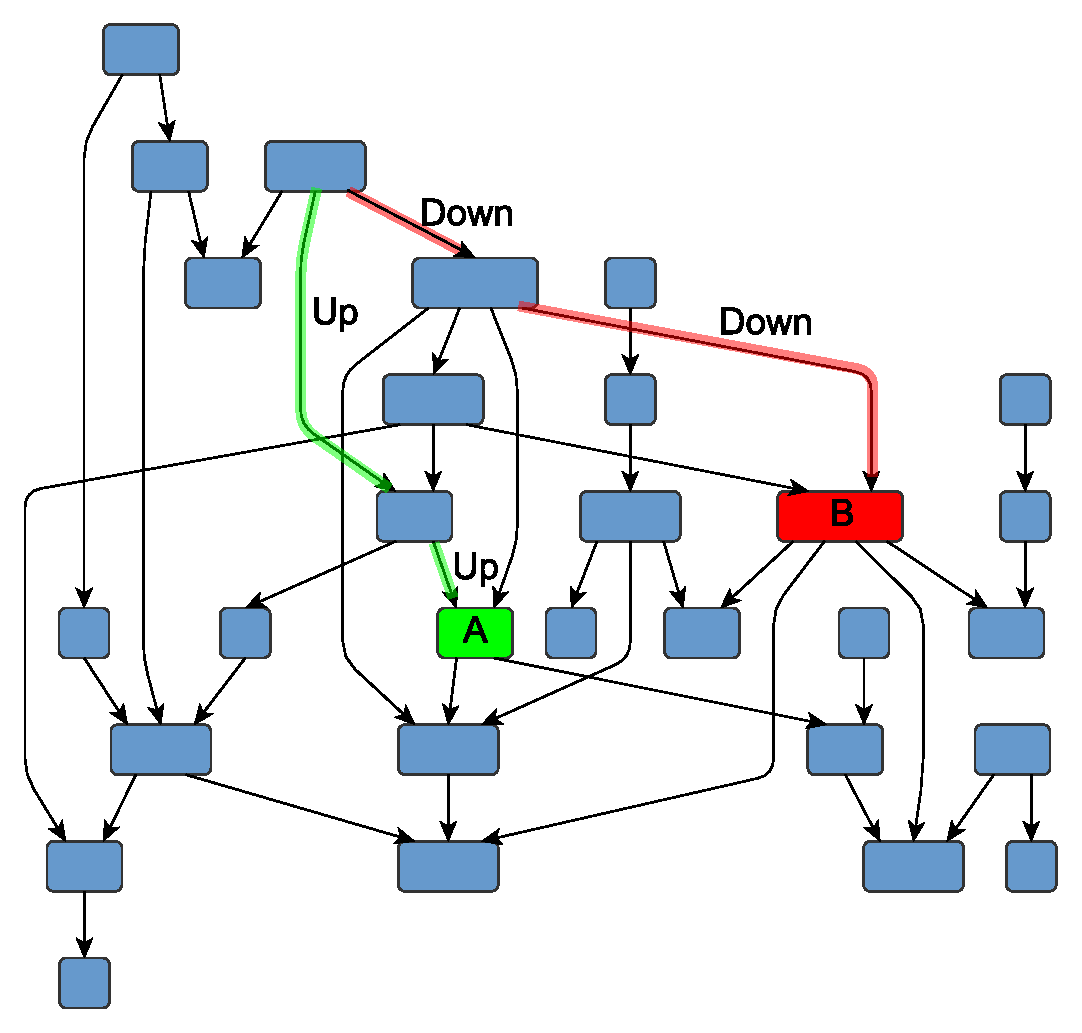
\includegraphics[width=\textwidth]{pictures/hierarchical.pdf}}
  \end{minipage}\hfill
  \begin{minipage}[m]{0.5\linewidth}
  Navigation through a graph
  \begin{itemize}
        \item Are nodes A and B on the same level of hierarchy?
        \item Is there a path of form $\textbf{Up}^n \, \textbf{Down}^n$?
        \item Find all paths of form $\textbf{Up}^n \, \textbf{Down}^n$ which start from the~node A
  \end{itemize}

  \end{minipage}

  \end{frame}

%  \begin{frame}[fragile] \frametitle{Applicatipons}
%    \begin{itemize}
%      \item Static code analysis
%      \item Graph database querying
%      \item RDF analysis
%    \end{itemize}
%  \end{frame}

  \begin{frame}[fragile]
    \frametitle{CFPQ: Query Semantics}
    \begin{itemize}
      \item $\mathbb{G} = (\Sigma, N, P)$ --- context-free grammar in normal form
      \begin{itemize}
        \item $A \rightarrow B C$, where $A, B, C \in N$
        \item $A \rightarrow x$, where $A \in N, x \in \Sigma \cup \{\varepsilon\}$
        \item $L(\mathbb{G},A) = \{ \omega \mid A \Rightarrow^* \omega \}$
      \end{itemize}
      \pause
      \item $G = (V,E,L)$ --- directed graph
        \begin{itemize}
          \item $v \xrightarrow{l} u \in E$
          \item $L \subseteq \Sigma$
        \end{itemize}
        \pause
      %\item $p = v_0 \xrightarrow{l_0} v_1 \xrightarrow{l_1} \cdots \xrightarrow{l_{n-2}} v_{n-1} \xrightarrow{l_{n-1}} v_n$ --- path in $G$
      \item $\omega(\pi) = \omega(v_0 \xrightarrow{l_0} v_1 \xrightarrow{l_1} \cdots \xrightarrow{l_{n-2}} v_{n-1} \xrightarrow{l_{n-1}} v_n) = l_0 l_1 \cdots l_{n-1}$
      \pause
      \item $R_A = \{ (n, m) \mid \exists n \pi m$, such that $\omega(\pi) \in L(\mathbb{G},A)\}$
    \end{itemize}
  \end{frame}

  \begin{frame}[fragile] \frametitle{CFPQ: Existing solutions}
    	\begin{itemize}
    		\item Solutions based on different parsing techniques (CYK, LL, LR, etc.)
    		\pause
    		\item Matrix-based solutions
    		\pause
    		\item All existing solutions work only with context-free grammar in normal form (CNF, BNF)
    		\pause
    		\item The transformation takes time and can lead to a significant grammar size increase
    		
    	\end{itemize}
  \end{frame}

\begin{frame}[fragile] \frametitle{Recursive State Machines (RSM)}
\begin{itemize}
	\item RSM behaves as a set of finite state machines (FSM) with additional recursive calls
	\item Any CFG can be easily encoded by an RSM with one box per nonterminal
\end{itemize}

\begin{figure}[h]
	\begin{tikzpicture}[shorten >=1pt,auto]
	\node[state, initial] (q_0)   {$q_S^0$};
	\node[state] (q_1) [right=of q_0] {$q_S^1$};
	\node[state] (q_2) [right=of q_1] {$q_S^2$};
	\node[state, accepting] (q_3) [right=of q_2] {$q_S^3$};
	\path[->]
	(q_0) edge node {a} (q_1)
	(q_1) edge node {S} (q_2)
	(q_2) edge node {b} (q_3)
	(q_1) edge [bend left = 38, above]  node {b} (q_3);
	\node[draw=black, fit= (q_0) (q_1) (q_2) (q_3), xshift=-4.5ex, inner sep=0.95cm, label=Box S] {};
	\end{tikzpicture}
	\centering
	\caption{The RSM for grammar with rules $S \to a S b \mid a b$}
\end{figure}

\end{frame}

\begin{frame}[fragile] \frametitle{CFPQ Algorithm Iteration 1}	

\begin{figure}[h]
	\centering
	\begin{subfigure}{.46\textwidth}
		\begin{center}
			\begin{tikzpicture}[shorten >=1pt,auto]
			\node[state] (q_0)                      {$0$};
			\node[state] (q_1) [right=of q_0]       {$1$};
			\node[state] (q_2) [right=of q_1]       {$2$};
			\node[state] (q_3) [right=of q_2]       {$3$};
			\path[->]
			(q_0) edge  node {a} (q_1)
			(q_1) edge  node {S} (q_2)
			(q_2) edge  node {b} (q_3)
			(q_1) edge[bend left = 45, above]  node {b} (q_3);
			\end{tikzpicture}
		\end{center}
	\end{subfigure}
\begin{subfigure}{.07\textwidth}
	\begin{center}
		\huge{$\otimes$}
	\end{center}
\end{subfigure}
	\begin{subfigure}{.36\textwidth}
		\begin{center}
			\begin{tikzpicture}[shorten >=1pt,auto]
			\node[state] (q_0)                      {$0$};
			\node[state] (q_1) [above right=of q_0] {$1$};
			\node[state] (q_2) [right=of q_0]       {$2$};
			\node[state] (q_3) [right=of q_2]       {$3$};
			\path[->]
			(q_0) edge  node {a} (q_1)
			(q_1) edge  node {a} (q_2)
			(q_2) edge  node {a} (q_0)
			(q_2) edge[bend left, above]  node {b} (q_3)
			(q_3) edge[bend left, below]  node {b} (q_2);
			\end{tikzpicture}
		\end{center}
	\end{subfigure}
\begin{subfigure}{.07\textwidth}
	\begin{center}
		\huge{$=$}
	\end{center}
\end{subfigure}

\pause

	\begin{subfigure}{.38\textwidth}
		\begin{center}
			\[
		\begin{array}{rcccl}
		0,0 & \xrightarrow{\text{a}} & 1,1 & & \\
		0,\underline{\textbf{1}} & \xrightarrow{\textbf{a}} & 1,2 & \xrightarrow{\textbf{b}} & 	3,\underline{\textbf{3}}\\
		0,2 & \xrightarrow{\text{a}} & 1,0 & & \\
		2,2 & \xrightarrow{\text{b}} & 3,3 & & \\
		2,3 & \xrightarrow{\text{b}} & 3,2 & & \\
		1,3 & \xrightarrow{\text{b}} & 3,2 & & \\
		\end{array}
		\]
		%\caption{Constructing the product automaton}
		\end{center}
	\end{subfigure}
\pause
\begin{subfigure}{.08\textwidth}
	\begin{center}
		\huge{$$\rightarrow$$}
	\end{center}
\end{subfigure}
	\begin{subfigure}{.48\textwidth}
		\begin{center}
			\begin{tikzpicture}[shorten >=1pt,auto]
			\node[state] (q_0)                      {$0$};
			\node[state] (q_1) [above right=of q_0] {$1$};
			\node[state] (q_2) [right=of q_0]       {$2$};
			\node[state] (q_3) [right=of q_2]       {$3$};
			\path[->]
			(q_0) edge  node {a} (q_1)
			(q_1) edge  node {a} (q_2)
			(q_1) edge[color=red, bend left, above]  node {\textbf{S}} (q_3)
			(q_2) edge  node {a} (q_0)
			(q_2) edge[bend left, above]  node {b} (q_3)
			(q_3) edge[bend left, below]  node {b} (q_2);
			\end{tikzpicture}
			%\caption{The updated input graph $\mathcal{G}$ using rule $S \to a b$}
		\end{center}
	\end{subfigure}


%\begin{itemize}
%	\item  We need to intersect these two graphs by constructing the product automaton
%\end{itemize}
	
\end{figure}

\end{frame}


\begin{frame}[fragile] \frametitle{CFPQ Algorithm Iteration 2}	

\begin{figure}[h]
	\centering
	\begin{subfigure}{.46\textwidth}
		\begin{center}
			\begin{tikzpicture}[shorten >=1pt,auto]
			\node[state] (q_0)                      {$0$};
			\node[state] (q_1) [right=of q_0]       {$1$};
			\node[state] (q_2) [right=of q_1]       {$2$};
			\node[state] (q_3) [right=of q_2]       {$3$};
			\path[->]
			(q_0) edge  node {a} (q_1)
			(q_1) edge  node {S} (q_2)
			(q_2) edge  node {b} (q_3)
			(q_1) edge[bend left = 45, above]  node {b} (q_3);
			\end{tikzpicture}			
		\end{center}
	\end{subfigure}
	\begin{subfigure}{.07\textwidth}
		\begin{center}
			\huge{$\otimes$}
		\end{center}
	\end{subfigure}
	\begin{subfigure}{.36\textwidth}
		\begin{center}
			\begin{tikzpicture}[shorten >=1pt,auto]
			\node[state] (q_0)                      {$0$};
			\node[state] (q_1) [above right=of q_0] {$1$};
			\node[state] (q_2) [right=of q_0]       {$2$};
			\node[state] (q_3) [right=of q_2]       {$3$};
			\path[->]
			(q_0) edge  node {a} (q_1)
			(q_1) edge  node {a} (q_2)
			(q_1) edge[bend left, above]  node {\textbf{S}} (q_3)
			(q_2) edge  node {a} (q_0)
			(q_2) edge[bend left, above]  node {b} (q_3)
			(q_3) edge[bend left, below]  node {b} (q_2);
			\end{tikzpicture}
		\end{center}
	\end{subfigure}
	\begin{subfigure}{.07\textwidth}
		\begin{center}
			\huge{$=$}
		\end{center}
	\end{subfigure}
	\pause
	\begin{subfigure}{.36\textwidth}
	\begin{center}
		\[
		\begin{array}{rcccccl}
		0,\underline{\textbf{0}} & \xrightarrow{\textbf{a}} & 1,1 & \xrightarrow{\textbf{S}} & 2,3 & \xrightarrow{\textbf{b}} & 3,\underline{\textbf{2}} \\
		0,1 & \xrightarrow{\text{a}} & 1,2 & \xrightarrow{\text{b}} &	3,3 & &\\
		0,2 & \xrightarrow{\text{a}} & 1,0 & & & &\\
		2,2 & \xrightarrow{\text{b}} & 3,3 & & & &\\
		1,3 & \xrightarrow{\text{b}} & 3,2 & & & &\\
		\end{array}
		\]
	\end{center}
\end{subfigure}
\pause
\begin{subfigure}{.07\textwidth}
	\begin{center}
		\huge{$$\rightarrow$$}
	\end{center}
\end{subfigure}
\begin{subfigure}{.55\textwidth}
	\begin{center}
		\begin{tikzpicture}[shorten >=1pt,auto]
		\node[state] (q_0)                      {$0$};
		\node[state] (q_1) [above right=of q_0] {$1$};
		\node[state] (q_2) [right=of q_0]       {$2$};
		\node[state] (q_3) [right=of q_2]       {$3$};
		\path[->]
		(q_0) edge  node {a} (q_1)
		(q_1) edge  node {a} (q_2)
		(q_1) edge[bend left, above]  node {\text{S}} (q_3)
		(q_2) edge  node {a} (q_0)
		(q_2) edge[bend left, above]  node {b} (q_3)
		(q_3) edge[bend left, below]  node {b} (q_2)
		(q_0) edge[color=red, bend right = 60, below]  node {\textbf{S}} (q_2);
		\end{tikzpicture}
	\end{center}
\end{subfigure}

	
\end{figure}

\end{frame}


\begin{frame}[fragile] \frametitle{CFPQ Algorithm: Kronecker Product}
%\begin{itemize}
	%\item We repeat these iterations while input graph $\mathcal{G}$ is changing
	Automaton intersection is a \textbf{Kronecker product} of adjacency matrices for $\mathcal{G}$ and $\mathcal{G}_{RSM}$
	{\scriptsize
	$$
	\begin{pmatrix}
    . & \{a\} & . & .     \\
    . & . & \{S\} & \{b\} \\
    . & . & . & \{b\}     \\
    . & . & . & .
    \end{pmatrix}
    \otimes
    \begin{pmatrix}
    . & \{a\} & . & .     \\
    . & . & \{a\} & .     \\
    \{a\} & . & . & \{b\} \\
    . & . & \{b\} & .
    \end{pmatrix}
    =$$
    }
    {\scriptsize
    \renewcommand{\arraystretch}{0.5}
    \setlength\arraycolsep{0.1pt}
    \begin{align*}
    & \kbordermatrix{
    	& (0,0) & (0,1) & (0,2) & (0,3) & \vrule & (1,0) & (1,1) & (1,2) & (1,3) & \vrule &  (2,0) & (2,1) & (2,2) & (2,3) & \vrule &  (3,0) & (3,1) & (3,2) & (3,3) &\\ 
    	(0,0) & . & . & . & . & \vrule & . & \{a\} & . & . & \vrule & . & . & . & . &  \vrule & . & . & . & . \\
    	(0,1) & . & . & . & . & \vrule & . & . & \mca & . & \vrule & . & . & . & . &  \vrule & . & . & . & . \\
    	(0,2) & . & . & . & . & \vrule & \{a\} & . & . & . & \vrule & . & . & . & . &  \vrule & . & . & . & . \\
    	(0,3) & . & . & . & . & \vrule & . & . & . & . & \vrule & . & . & . & . &  \vrule & . & . & . & . \\
    	\hline
    	(1,0) & . & . & . & .  & \vrule & . & . & . & . & \vrule & . & . & . & . & \vrule & . & . & . & . \\
    	(1,1) & . & . & . & .  & \vrule & . & . & . & . & \vrule & . & . & . & . & \vrule & . & . & . & . \\
    	(1,2) & . & . & . & .  & \vrule & . & . & . & . & \vrule & . & . & . & . & \vrule & . & . & . & \mcb \\
    	(1,3) & . & . & . & .  & \vrule & . & . & . & . & \vrule & . & . & . & . & \vrule & . & . & \{b\} & . \\
    	\hline
    	(2,0) & . & . & . & .  & \vrule & . & . & . & . & \vrule & . & . & . & . & \vrule & . & . & . & . \\
    	(2,1) & . & . & . & .  & \vrule & . & . & . & . & \vrule & . & . & . & . & \vrule & . & . & . & . \\
    	(2,2) & . & . & . & .  & \vrule & . & . & . & . & \vrule & . & . & . & . & \vrule & . & . & . & \{b\} \\
    	(2,3) & . & . & . & .  & \vrule & . & . & . & . & \vrule & . & . & . & . & \vrule & . & . & \{b\} & . \\
    	\hline
    	(2,0) & . & . & . & .  & \vrule & . & . & . & . & \vrule & . & . & . & . & \vrule & . & . & . & . \\
    	(2,1) & . & . & . & .  & \vrule & . & . & . & . & \vrule & . & . & . & . & \vrule & . & . & . & . \\
    	(2,2) & . & . & . & .  & \vrule & . & . & . & . & \vrule & . & . & . & . & \vrule & . & . & . & . \\
    	(2,3) & . & . & . & .  & \vrule & . & . & . & . & \vrule & . & . & . & . & \vrule & . & . & . & . \\
    }
    \end{align*}
}
	%\item We can use the sparse and block nature of the obtained matrices to apply wide class of optimizations
%\end{itemize}
\end{frame}

\begin{frame}[fragile] \frametitle{Implementations}

\begin{itemize}
	\item $\textbf{Kron}$ --- implementation of the proposed algorithm using \textbf{SuiteSparse} C implementation of \textbf{GraphBLAS} API, which provides a set of sparse matrix operations
	\pause
	\item We compare our implementation with $\textbf{Orig}$ --- the best CPU implementation of the original matrix-based algorithm using M4RI library
\end{itemize}
\end{frame}

\begin{frame} \frametitle{Evaluation}
\begin{itemize}
	\item OS: Ubuntu 18.04
	\item CPU: Intel(R) Core(TM) i7-4790 CPU 3.60GHz
	\item RAM: DDR4 32 Gb
\end{itemize}
\end{frame}


\begin{frame}[fragile] \frametitle{Evaluation results\footnote{Queries are based on the context-free grammars for 
		nested parentheses} \footnote{Time is measured in seconds}}
\begin{center}
	\tikzmark{yyy}{
	}
 {\small
 \setlength{\tabcolsep}{0.35em}
 			\centering
 			\label{tbl:tableRDF}
 			%\rowcolors{1}{}{lightgray}
 			\begin{tabular}{| c | p{1.6cm} | c | c | c | c || c | p{0.8cm} | c | c | c | c |}
 				\hline
 				&  Graph              & \#V & \#E  & $Kron$  & $Orig$ &  & Graph & \#V & \#E     & $Kron$    & $Orig$ \\
 				\hline
 				\hline
 				\parbox[t]{2mm}{\multirow{11}{*}{\rotatebox[origin=c]{90}{RDF}}}
 				& \small{generations}                 & 129 & 351     & 0.04  & 0.03 &
 				\parbox[t]{2mm}{\multirow{2}{*}{\rotatebox[origin=c]{90}{RDF}}} & \small{core}                        & 1323 & 8684   & 0.28  &  0.12   \\
 				& \small{travel}                      & 131 & 397     & 0.05  & 0.05 & & \small{pways}                    & 6238 & 37196  & 4.88 &   0.18      \\\cline{7-12}
 				& \small{skos}                        & 144 & 323     & 0.02  & 0.04 &
 				\parbox[t]{2mm}{\multirow{5}{*}{\rotatebox[origin=c]{90}{Worst case}}} & $WC_1$& 64 & 65 & 0.03 & 0.04      \\
 				& \small{unv-bnch}                    & 179 & 413     & 0.05  & 0.04 & & $WC_2$ & 128 & 129 & 0.16 & 0.23      \\
 				& \small{foaf}                        & 256 & 815     & 0.07  & 0.02  & & $WC_3$ & 256 & 257 & 0.96 & 1.99    \\
 				& \small{atm-prim}                    & 291 & 685     & 0.24   & 0.02 & & $WC_4$ & 512 & 513 & 7.14 & 23.21      \\
 				& \small{ppl\_pets}                & 337 & 834     & 0.18  & 0.03 & & $WC_5$ & 1024& 1025&  121.99 & 528.52      \\ \cline{7-12}
 				& \small{biomed}                      & 341 & 711     & 0.24  & 0.05 &
 				\parbox[t]{2mm}{\multirow{4}{*}{\rotatebox[origin=c]{90}{Full}}} & $F_1$ & 100 & 100 & 0.17 &  0.02     \\
 				& \small{pizza}                       & 671 & 2604    & 1.14  & 0.08 & & $F_2$ & 200 & 200 & 1.04 & 0.03        \\
 				& \small{wine}                        & 733 & 2450    & 1.71  & 0.06 & & $F_3$ & 500 & 500 & 18.86  & 0.03   \\
 				& \small{funding}                     & 778 & 1480    & 0.43  & 0.07  & & $F_4$ & 1000 & 1000& 554.22 & 0.07       \\
 				\hline
 			\end{tabular}
 	}
\end{center} 
\pause
\onslide<2>{\tikz[overlay,remember picture]{\draw[draw=red,thick,fill opacity=0.2] ($ (yyy) + (-1.65,-0.6)$) rectangle ($ (yyy) + (0.08,-2.2)$);}}
\pause
\onslide<3>{\tikz[overlay,remember picture]{\draw[draw=red,thick,fill opacity=0.2] ($ (yyy) + (3.98,-3.55)$) rectangle ($ (yyy) + (6.2,-5.15)$);}}
\pause
\onslide<4>{\tikz[overlay,remember picture]{\draw[draw=red,thick,fill opacity=0.2] ($ (yyy) + (3.98,-1.45)$) rectangle ($ (yyy) + (6.25,-3.45)$);}}
\end{frame}

\begin{frame}[fragile] \frametitle{Conclusion}
  \begin{itemize}
  	\item We show that the linear algebra based CFPQ can be done without grammar transformation
  	\pause
  	\item The Kronecker product can be used as the main matrix operation in such algorithm
  	\pause
  	\item We show that in some cases our algorithm outperforms the original matrix-based algorithm
  	%\pause
    %item We can use existing high-performance libraries for matrix operations
  \end{itemize}
\end{frame}

\begin{frame}[fragile] \frametitle{Future Research}
  \begin{itemize}
  	\item Improve our implementation to make it applicable for real-world graphs analysis
  	\pause
  	\item Analyze how the behavior depends on the query type and its form
  	\begin{itemize}
  		\item Analyze regular path queries evaluation and context-free path queries in the form
  		of extended context-free grammars (ECFG)
  	\end{itemize}
  	\pause	
    \item Compare our algorithm with the matrix-based one
    in cases when the size difference between Chomsky Normal Form and ECFG
    representation of the query is significant
    \pause
    \item Extend our algorithm to single-path and all-path
    query semantics
\end{itemize}
\end{frame}

\begin{frame}
\frametitle{Contact Information}
\begin{itemize}
  \item Semyon Grigorev:
    \begin{itemize}
      \item \href{mailto:s.v.grigoriev@spbu.ru}{s.v.grigoriev@spbu.ru}
      \item \href{mailto:Semen.Grigorev@jetbrains.com}{Semen.Grigorev@jetbrains.com}
    \end{itemize}
  \item Rustam Azimov:
  \begin{itemize}
  	\item \href{mailto:rustam.azimov19021995@gmail.com}{rustam.azimov19021995@gmail.com}
  	\item \href{mailto:Rustam.Azimov@jetbrains.com}{Rustam.Azimov@jetbrains.com}
  \end{itemize}
  \item Egor Orachev: \href{mailto:egor.orachev@gmail.com}{egor.orachev@gmail.com}
  \item Ilya Epelbaum: \href{mailto:iliyepelbaun@gmail.com}{iliyepelbaun@gmail.com}
\vspace{0.5cm}
  \item Dataset: \href{https://github.com/JetBrains-Research/CFPQ_Data}{https://github.com/JetBrains-Research/CFPQ\_Data}
   \item Algorithm implementations: \href{https://github.com/YaccConstructor/RedisGraph}{https://github.com/YaccConstructor/RedisGraph}
\end{itemize}
\vspace{0.1cm}
\center{\huge{Thanks!}}
\end{frame}
\end{document}
